\chapter{Jaynes-Cummings de dos átomos, no lineal, medio Kerr}
\label{ch4_dinamica}

%CAMBIAR ESTO PARA PERSONALIZARLO A MI GUSTO
\pagestyle{fancy}
\fancyhf{}
\fancyhead[LE]{\nouppercase{\rightmark\hfill}}
\fancyhead[RO]{\nouppercase{\leftmark\hfill}}
\fancyfoot[LE,RO]{\hfill\thepage\hfill}

En este capitulo se extiende el modelo de Jaynes-Cummings presentado en el capitulo \ref{ch3_jcm}, agregandole nuevas cosas. Lo mas importante es que ahora vamos a tener dos átomos dentro de una misma cavidad. En la literatura en general, el JCM fue extendido para considerar dos cavidades donde cada una tiene su propio átomo, y usando una condición inicial entrelazada se puede hacer interactuar ambas cavidades REFS. El camino que se tomó en este trabajo, es un tanto fuera de lo convensional ya que no hay muchos estudios sobre este sistema. El principal obstaculo que presenta este problema, es que el espacio de Hilbert crece mucho y se torna inmanejable analiticamente; como bien ya sabemos, el JCM tiene subespacios de 2 dimensiones que no se mezclan, y utilizando esta estrategia vamos a ver que en este caso tenemos subespacios de 4x4 que tampoco se mezclan en el caso unitario. Esto nos permite encontrar algunas expresiones analiticas, pero en general se utilizaran métodos númericos para analizar la dinamica. \newline
Este capitulo entonces seguira un hilo conductor, partiendo desde el caso mas sencillo hasta llegar a analizar cuales son los efectos de los diferentes parámetros en el problema. 
	Primero vamos a considerar una cavidad perfecta, es decir sin disipaci\'on, agregandole el segundo átomo, vamos a intentar de entender cual es el efecto de este sobre el modelo de un solo átomo. Para esto haremos un analisis poblacional, y de observables como la entropia reducida, la concurrencia, las matrices de pauli. Una vez agregado el segundo átomo, vamos a prender las interacciones de a una y vamos a analizar cuales son sus efectos. Luego, vamos a comparar esto con el caso en donde la cavidad presenta perdidas. Principalmente, nos centraremos en un analisis del entrelazamiento, ya que esta es la cualidad mas interesante que tenemos en el ambito de la informaci\'on cu\'antica. 

\textcolor{blue}{Luego, se analizar\'a el problema para dos átomos, primero en el caso que estos no interact\'uan
directamente entre si, sino que lo hace indirectamente a travez de la cavidad. La comparativa entre
esta situación y la mas comun, donde los átomos interactuan mediante sus espines o sus momentos
dipolares, es muy rica porque nos permite discernir con claridad cual es el efecto de la cavidad
y cual de la interacción entre los átomos a la hora de entrelazarse e intercambiar energía.
El problema de dos átomos tiene una peculiaridad al elegir las condiciones iniciales, ya que la
dinamica depende de esta eleccion, y hay muchas diferentes configuraciones interesantes, por un lado
por la gran dimension del espacio, y por otro lado, esta la posibilidad de jugar con las simetrias.
Surge asi la pregunta de si es importante, o si tiene sentido, teniendo dos átomos indistinguibles
en una cavidad, que la condición inicial sea asimetrica ante intercambio. 
}

\section{JCM de dos átomos}
En este trabajo, nos vamos a concentrar en una extension del modelo, donde vamos a ubicar dos átomos dentro de la cavidad. Estos átomos pueden interactuar entre si, y con la cavidad, y ademas agregaremos no-linealidades en el acoplamiento y en el medio.
Vamos a usar un modelo de Jaynes-Cummings para describir la interacci\'on entre el campo electromagn\'etico y los átomos. Adem\'as supondremos que el acoplamiento depende de la cantidad de fotones y los átomos podr\'an interactuar entre si mediante un termino tipo Ising y otro tipo dipolo-dipolo. Recordemos que para estamos asumiendo que vale la aproximaci\'on de onda rotante ($\omega_0 \sim \omega$) y $g << \omega,\omega_0$.
Entonces, el Hamiltoniano que describe este problema es el siguiente:

\begin{equation}
\begin{split}
     \hat H & =\underbrace{\hbar \omega_0 h(\hat n) \hat n }_{\hat H_F}+\underbrace{\frac{\hbar \omega}{2}(\hat\sigma_Z^{(1)}+\hat\sigma_Z^{(2)})}_{\hat H_A}   \\ 
     & + \underbrace{\hbar g(\hat\sigma_+^{(1)}\hat a f(\hat n)+\hat\sigma_-^{(1)}f(\hat n) \hat a^\dagger + \hat\sigma_+^{(2)}\hat a f(\hat n)+\hat\sigma_-^{(2)}f(\hat n) \hat a^\dagger)}_{H_{FA}} + \\ & \underbrace{2\hbar \kappa (\hat \sigma_-^{(1)}\hat \sigma_+^{(2)}+\hat \sigma_+^{(1)}\hat \sigma_-^{(2)}) + \hbar J \hat \sigma_Z^{(1)}\hat \sigma_Z^{(2)}}_{H_{AA}}
\end{split}
\end{equation}

donde $\hat a$ es el operador de aniquilaci\'on del fot\'on, $\omega_0$ y $\omega$ son las frecuencias del fot\'on y del átomo respectivamente, $g$ es la constante de acoplamiento, las constantes $J$ y $\kappa$ son los par\'ametros de Ising y de dipolo-dipolo para las interacciones átomo-átomo, y los operadores $\sigma^{(i)}$ son las matrices de Pauli que act\'uan sobre el átomo i-esimo. Finalmente, las funciones $h(\hat n)$ y $f(\hat n)$ son las que van a dar cuenta de la no linealidad dependiente del numero de fotones de la cavidad $\hat n = \hat a^\dagger \hat a$. 

Tomando un medio tipo Kerr la funci\'on $h(\hat n)=1+\frac{\chi}{\omega_0}\hat n$ \cite{}\textcolor{red}{(CITA)}, y la funci\'on $f(\hat n) =1$ si tomamos un acoplamiento lineal, y $f(\hat n) = \sqrt{\hat n}$ si consideramos un acoplamiento tipo Buck-Sukumar \cite{}\textcolor{red}{(CITA)}

En este punto es normal hacer una transformaci\'on unitaria  $K = \exp\left\{-i \omega t (\hat a^\dagger a + \sigma_z/2)\right\}$ para dejar el Hamiltoniano en funci\'on del Detuning $\Delta (\sim 0)$. 

\begin{equation}
\begin{split}
     \hat H_I & =\hbar \chi \hat n^2+\frac{\hbar \Delta}{2}(\hat\sigma_Z^{(1)}+\hat\sigma_Z^{(2)})   \\ 
     & + \hbar g(\hat\sigma_+^{(1)}\hat a f(\hat n)+\hat\sigma_-^{(1)}f(\hat n) \hat a^\dagger + \hat\sigma_+^{(2)}\hat a f(\hat n)+\hat\sigma_-^{(2)}f(\hat n) \hat a^\dagger) \\ 
 & + 2\hbar \kappa (\hat \sigma_-^{(1)}\hat \sigma_+^{(2)}+\hat \sigma_+^{(1)}\hat \sigma_-^{(2)}) + \hbar J \hat \sigma_Z^{(1)}\hat \sigma_Z^{(2)}
\end{split}
\end{equation}
Este es el Hamiltoniano con el que vamos a trabajar, asi que a partir de ahora vamos a olvidarnos del subindice I. Obsérvese que el caso de $\chi=0$ es el caso de un medio lineal. 
ACA PUEDO AGREGAR UN ESQUEMA DE COMO SERIA. En este esquema se ve como seria el experimento planteado. 

Este Hamiltoniano se puede resolver analiticamente para el caso de una cavidad sin perdidas. En analogia con el caso de 1 átomo, vamos a elegir la base de N excitaciones, donde esperamos que estos subespacios queden invariantes, es decir, que el Hamiltoniano sea diagonal por bloques, pero como ahora tenemos 2 átomos, tenemos que elegir una base que respete simetrias, para N excitaciones los estados de la base son $\left\{\ket{ggn},\frac{1}{\sqrt{2}}(\ket{eg,n-1}+\ket{ge,n-1}),\ket{ee,n-2},,\frac{1}{\sqrt{2}}(\ket{eg,n-1}-\ket{ge,n-1})\right\}$. En esta base, el Hamiltoniano se diagonaliza por bloques y el bloque de N excitaciones queda
El problema unitario se puede resolver analíticamente. Esto esta hecho en el paper de los autores \textit{O de los Santos-Sánchez
, C González-Gutiérrez and J Récamier}, titulado \textit{Nonlinear Jaynes–Cummings model for two
interacting two-level atoms} \cite{paper:santos}\textcolor{red}{(CITA)}. 
\textcolor{red}{Ac\'a tengo que pasar las cuentas a latex, pero las hice en papel para ver si entend\'ia todo.}
Para resolver el problema lo primero que hacemos es notar que el Hamiltoniano conserva el numero de exitaciones, es decir $[H,\hat N]=0$, y en esta situación es sabido que el Hamiltoniano de JC es diagonal por bloques si elegimos convenientemente la base, esta es la que agrupa los estados con misma cantidad de excitaciones $\hat N = \hat n + \hat \sigma_+^{(1)}\hat \sigma_-^{(1)}+\hat \sigma_+^{(2)}\hat \sigma_-^{(2)}$: 
\begin{equation}
\begin{split}
    & \left\{\ket{\Phi^{(n)}_1}=\ket{ggn},\ket{\Phi^{(n)}_2}=\frac{1}{\sqrt{2}}(\ket{egn-1}+\ket{gen-1}),\ket{\Phi^{(n)}_3}=\ket{een-2},\right. \\
& \left. \ket{\Phi^{(n)}_4}=\frac{1}{\sqrt{2}}(\ket{egn-1}-\ket{gen-1})\right\} 
\end{split}
\end{equation}
,donde se eligi\'o esta combinaci\'on particular porque el ultimo estado de la base, que es impar ante intercambio, queda desacoplado de los otros, simplificando el problema. Esto se ve al evaluar los elementos de matriz del Hamiltoniano $H_{i,j}=\bra{\Phi_i}\hat H \ket{\Phi_j}$, este queda en bloques, y el subespacio correspondiente a $n$ excitaciones $\hat H^{(n)}$ es una matriz de 4x4
\begin{equation}
    \hat H^{(n)} = 
    \begin{pmatrix}
    \hbar \chi n^2 - \hbar \Delta + \hbar J & \sqrt{2}\hbar g f(n)\sqrt{n} & 0 & 0 \\
    \sqrt{2}\hbar g f(n)\sqrt{n} & \hbar \chi (n-1)^2  - \hbar J + 2\hbar k & \sqrt{2}\hbar g f(n-1)\sqrt{n-1} & 0 \\
    0 & \sqrt{2}\hbar g f(n-1)\sqrt{n-1} & \hbar \chi (n-2)^2 + \hbar \Delta + \hbar J & 0 \\
    0&0&0&\hbar \chi (n-1)^2 - \hbar \Delta - 2\hbar k
    \end{pmatrix}
\end{equation}
Vemos claramente que el estados impar ante intercambio esta aislado, y entonces es autoestado del problema, y por lo tanto evoluciona solo y no se mezcla con los otros estados. Esto nos sirve porque ahora, para terminar de resolver el problema, tenemos que diagonalizar la matriz de 3x3. Cabe aclarar que esta matriz solo es valida para $n\geq 2$, ya que los subespacios con $N=0,1$ no tienen 4 estados. En estos casos la soluci\'on del problema de autovalores es mas sencilla aun, as\'i que solo dejaremos los resultados. A partir de ahora se usar\'a como convención $\hbar=1$. \newline
Para resolver el problema de autovalores de la matriz de 3x3 utilizamos la fórmula de Cardano para conseguir las ra\'ices triples que nos aparecen en el polinomio caracter\'istico, y entonces encontramos que los autovalores son
\begin{equation}
    E_j^{(n)}=-\frac{1}{3}\beta_n+2\sqrt{-Q_n}\cos{\left(\frac{\theta_n+2(j-1)\pi}{3}\right)}
\end{equation}
para $j=1,2,3$, y donde 
\begin{equation}
    \theta_n=\cos^{-1}\left(\frac{R_n}{\sqrt{-Q_n^3}}\right)
\end{equation}
\begin{align*}
    Q_n & = \frac{3\gamma_n-\beta_n^2}{9} \\
    R_n & = \frac{9\beta_n\gamma_n-27\eta_n-2\beta_n^3}{54} \\
    \beta_n & = - \left( \chi(n^2+(n-1)^2+(n-2)^2)+J+2k\right) \\
    \gamma_n & = (\chi(n-1)^2 - J + 2k)(x(n-2)^2+\chi n^2+2J) \\ 
    & +(\chi (n-2)^2+\Delta+J)(x n^2-\Delta+J)-2g^2(n^{2a}+(n-1)^{2a}) \\ 
    \eta_n &= -(\chi n^2-\Delta+J)(\chi(n-2)^2+\Delta+J)(\chi(n-1)^2-J+2k) \\
    &+2g^2 \left[  \chi(n-2)^2n^{2a}+\chi n^2(n-1)^{2a}+\Delta\left(n^{2a}-(n-1)^{2a}\right) +J(n^{2a}-(n-1)^{2a})\right]
\end{align*}
donde $a=\frac{1}{2}$ se corresponde con acoplamiento lineal, es decir, $f(n)=1$, y $a=1$ a Buck-Sukumar $f(n)=\sqrt{n}$. Los autovalores ser\'an reales si $Q_n^3+R_n^2<0$.
Con esto podemos escribir los autovectores:
\begin{equation}
    \begin{split}
        \ket{u_j^{(n)}} &= \frac{1}{N_j^{(n)}} \bigg[ \left((E_j^{(n)} - H_{22}^{(n)})(E_j^{(n)}-H_{33}^{(n)}) - H_{23}^{(n)^2} \right) \ket{\Phi_1^{(n)}} \\ &+ H_{31}^{(n)}(E_j^{(n)}-H_{33}^{(n)})\ket{\Phi_2^{(n)}} + H_{23}^{(n)}H_{12}^{(n)}\ket{\Phi_3^{(n)}}\bigg]
    \end{split}
\end{equation}
Obviamente no nos olvidemos del estado $\ket{\Phi_4^{(n)}}$, que tambi\'en es autoestado, con autovalor $E_4^{(n)}=\chi(n-1)^2-J-2k$.
Para el subespacio de $N=0$ solo tenemos un vector $\ket{\Phi_1^{(0)}}=\ket{gg0}$ y su autovalor es $E_1^{(0)}=-\Delta+J$.
Para $N=1$ tenemos 3 vectores en el subespacio, y las autoenergias son
\begin{align}
    E_{1,2}^{(1)} &=\frac{\chi -\Delta}{2} +k \pm \sqrt{2g^2+(k-J+\frac{\Delta -\chi}{2} )^2} \\
    E_3^{(1)} & = -2k-J 
\end{align}
y sus autovectores
\begin{align}
    \ket{u_{1,2}^{(1)}}&=\frac{1}{N_{1,2}^{(1)}}(-\sqrt{2}g\ket{gg1}+ \left(\frac{\chi-\Delta}{2}+J-k \mp \sqrt{2g^2+(k-J+\frac{\Delta -\chi}{2} )^2} \right)\dfrac{\ket{eg0}+\ket{ge0}}{\sqrt{2}}\\
    \ket{u_3^{(1)}}&= \frac{1}{\sqrt{2}}(\ket{eg0}-\ket{ge0})
\end{align}
Con esto, podemos resolver analíticamente la evolución temporal de cualquier estado inicial.
Para esto solo tenemos que desarrollar el estado inicial en terminos de los autovectores, y la evolución temporal esta dada por
\begin{equation}
\ket{\psi(t)}=e^{-iHt}\ket{\psi(0)}=\sum_{j,n} c_j^{(n)}e^{-iE_j^{(n)}t}\ket{u_j^{(n)}}
\end{equation}
donde $c_j^{(n)}=\braket{u_j^{(n)}}{\psi(0)}$.
La complejidad de estas expresiones hace complicado conseguir conclusiones interesantes,aun asi, algo que se puede notar, es la diferencia fundamental que se encuentra para las energias con un numero total de excitaciones $N=1$ y $N>1$. Si se observa el factor que esta antes de la raiz cuadrada,  se ve que para el caso en que $N \geq 2$ tenemos un $\frac{1}{3}\beta_n$ que solo depende de $\chi$, $J$, $k$ y $n$. Mientras tanto, en el caso de $N=1$, este factor depende del detunning $\Delta$. Esto es interesante, ya que uno podria pensar que la formula para $N$ excitaciones se puede generalizar para incluir $N=0,1$, pero la fundamental diferencia de tener mas o menos estados que interactuan entre si, da lugar a efectos fundamentalmente diferentes. Si uno mira en detalle las cuentas, se percata de que en el caso de $N=1$ este factor $\Delta$ aparece, ya que en la matriz Hamiltoniana el unico estado con $N=1$ que tiene un termino que incluye al detunning, es el estado $\ket{gg1}$, y los otros dos estados al ser un átomo excitado y otro no, el termino de detunning se cancela. Por lo tanto, este termino con $\Delta$ sobrevive, al contrario que en todos los demas subespacios, ya que tenemos por un lado el termino del $\ket{ggn}$ que nos aporta un $\Delta$, y el termino de $\ket{ee,n-2}$ que nos aporta otro $\Delta$ pero con el signo cambiado, y elimina la contribución del primer estado a la energía. Esto es super interesante, ya que para $N=1$, si aumentamos el detunning, no solo se separan los niveles de energía, sino que tambien hay una asimetria por el termino independiente. Para analizar esto en detalle, en la figura \ref{fig:relación energia detunning} se observan las energias de los diferentes niveles en función del detunning. 

\begin{figure}
    \centering
    \begin{subfigure}[h]{0.49\textwidth}
        \centering
        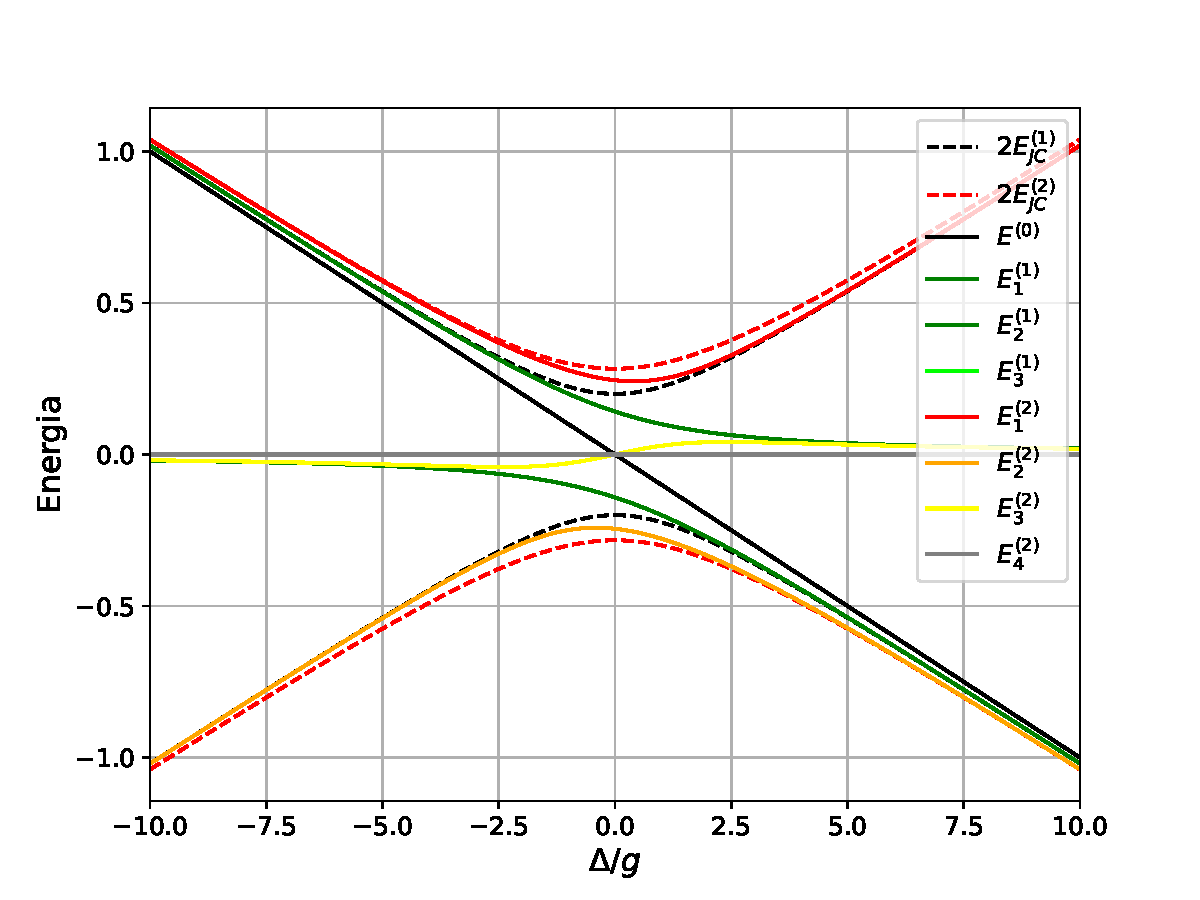
\includegraphics[width=\textwidth]{figuras/ch4/relacion_energia_detunning1.pdf}
        \caption{$k=J=0$}
        \label{fig:relación energia detunning 1}
    \end{subfigure}
    \hfill
    \begin{subfigure}[h]{0.49\textwidth}
        \centering
        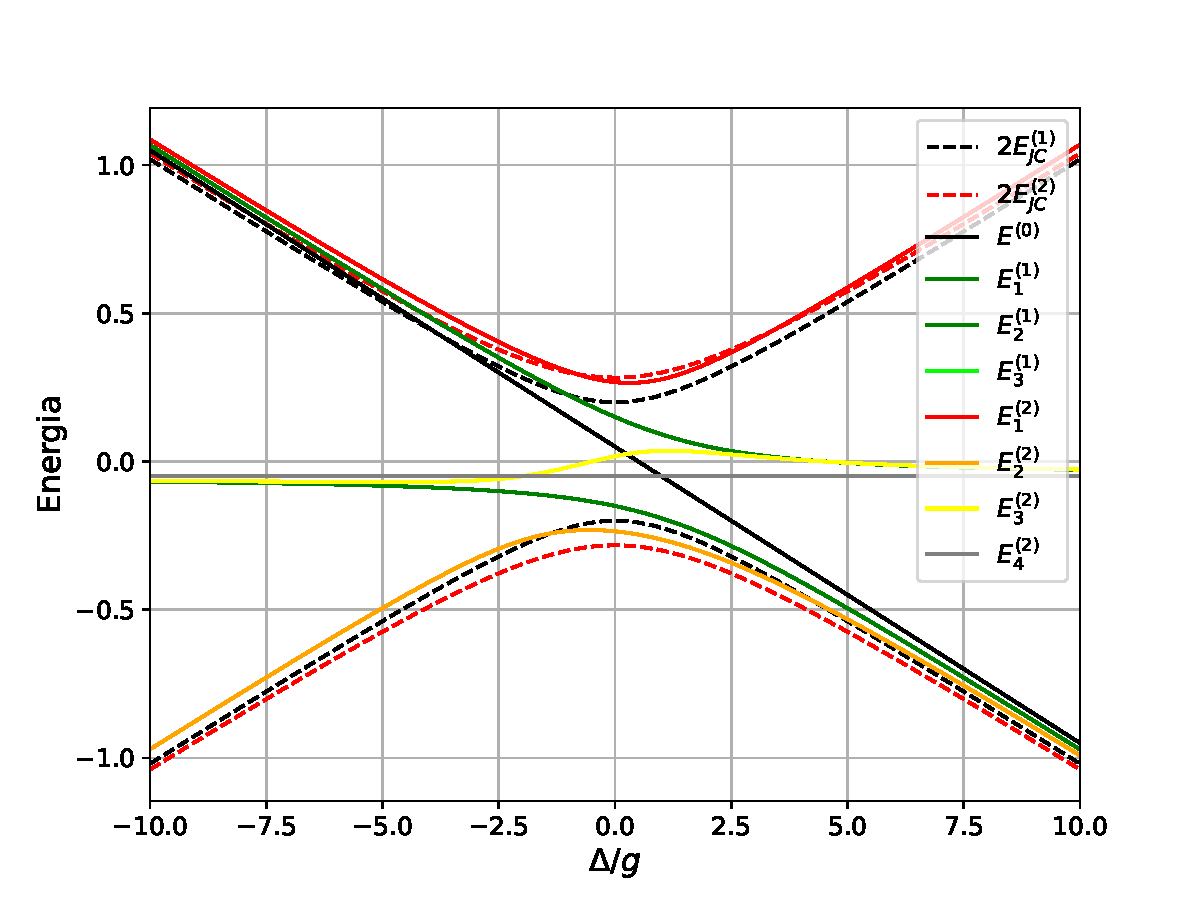
\includegraphics[width=\textwidth]{figuras/ch4/relacion_energia_detunning2.pdf}
        \caption{$J\neq 0$}
        \label{fig:relación energia detunning 2}
    \end{subfigure}
       \caption{Relación entre energía y detunning para los diferentes niveles de energía del problema. Las lineas solidas muestran la energía de los estados del JC doble con N=0 (negro, solido), N=1 (verde oscuro y lima, solido) y N=2 (rojo, naranja, amarillo y gris; solido). Tambien se muestran los niveles de energía del JC de un átomo para N=1 (negro; rayado) y N=2 (rojo; rayado). Observese que las energias del JC de un átomo estan multiplicadas por 2.}
       \label{fig:relación energia detunning}
\end{figure}
En esta figura \ref{fig:relación energia detunning 1} se observan las energias de los primeros niveles para el modelo de un átomo, mostrados con lineas rayadas, y de dos átomos, con lineas solidas; para esta figura se tomaron átomos que no interactuan ($k=J=0$) y una cavidad lineal ($\chi=0$). Se puede ver que, si bien el modelo de dos átomos tiene estructuras mas complicadas, son similares a las de 1 átomo. En primer lugar, los estados con N=2 (rojo y naranja; solido) tienen una forma igual a la de JC de 1 átomo, si bien esta un poco desfasada, es interesante ver como las lineas tienen una coincidencia muy grande, recordando que en el grafico las lineas rayadas estan multiplicadas por 2, esto nos da una interpretación bastante buena, y es que la energía de dos átomos no interactuantes en una cavidad es igual (o muy parecida) a dos veces la energía de 1 átomo en una cavidad. \textcolor{red}{Esto tengo que chequear con cuentas} Creo que esto se debe al corrimiento Lamb, ya que ahora tenemos dos átomos que interactuan con el vacio, entonces el corrimiento es 1 unidad mas grande en los extremos, que es justamente lo que vemos en el grafico, cuando el detunning es muy negativo, la energ\'ia tiende a ser igual a la de un JC simple con 2 excitaciones, y cuando el detunning es muy positivo, entonces tiende a la de 1 excitaci\'on; esta asimetr\'ia para $\Delta>0$ y $\Delta<0$ se observar\'a en resultados posteriores. Por otro lado, se puede observar lo que se habia comentado anteriormente, que la energ\'ia de los estados con $N=1$ tienen un t\'ermino fuera de la raiz, que hace que sea mas asim\'etrico a\'un. Normalmente, en el JC de 1 átomo, ya que todos los niveles de energía tienen una forma funcional igual, este termino de afuera de la raiz se le puede agregar o quitar como un offset en la energía del estado fundamental, la diferencia con este caso es que, no todos los niveles de energía presentan esto, entonces si agregamos un offset, igualmente habria una diferencia. 

Otra cosa interesante de notar es que si la cavidad es lineal, entonces los estados antisimetricos estan degenerados en energía.

Una vez estudiados los niveles de energía y comparados con el caso de 1 átomo, vamos a proseguir con la dinamica del problema, que en el caso unitario puede resolverse analiticamente, pero a\'un asi, nos concentraremos en simulaciones numericas.
Para comenzar, vamos a intentar de recuperar el caso de un átomo, asimetrizando el acoplamiento uno de los dos átomos que tenemos en la cavidad, y haciendo tender este a cero, es decir, vamos a trabajar con $k=J=0$ y vamos a agregar un parámetro adimensional $\alpha$ que solamente actua sobre el átomo 2, y sirve de apantallamiento. 

